Table~\ref{tab:occupation_accuracy} reports several regression where the outcome variable is the MSE in prediction, in log points. 
In Column~(1), we can see, unsurprisingly, that prediction errors are decreasing in the total employment in that population. 
Column~(2) adds as a predictor and indicator for whther the respondent knows that the job consists of. 
This is also negative, as expected, and lowers the employment coefficient.  
Column~(3) adds the social index predictor, which is negative (albeit not significant) lowers the employment and job knowledge coefficients. 
Finally, in Column~(4), we add the log mean hourly wage. 
It is strongly positive---consistent with our graphical evidence---and it also flips the sign of the employment coefficient.  
It also dramatically increases the adjusted $R^2$ of the regression. 
In the data, actual occupational wages and employment share have a strong negative correlation, which this sign-reversal reflects. 


% Table created by stargazer v.4.5.3 by Marek Hlavac, Harvard University. E-mail: hlavac at fas.harvard.edu
% Date and time: Tue, Dec 17, 2013 - 05:02:38 AM
\begin{table}[!htbp] \centering 
  \caption{Occupation attributes and worker accuracy} 
  \label{tab:occupation_accuracy} 
\begin{tabular}{@{\extracolsep{5pt}}lcccccc} 
\\[-1.8ex]\hline 
\hline \\[-1.8ex] 
 & \multicolumn{6}{c}{\textit{Dependent variable:}} \\ 
\cline{2-7} 
\\[-1.8ex] & \multicolumn{3}{c}{mse.wage} & \multicolumn{3}{c}{mse.v.trend} \\ 
\\[-1.8ex] & (1) & (2) & (3) & (4) & (5) & (6)\\ 
\hline \\[-1.8ex] 
 log(tot.emp) & $-$0.088 & 0.064 & 0.480 & 0.024 & 0.021 & $-$0.016 \\ 
  & (0.081) & (0.065) & (0.381) & (0.043) & (0.045) & (0.265) \\ 
  & & & & & & \\ 
 log(avg.wage) &  & 0.720$^{***}$ & 2.698 &  & $-$0.012 & $-$0.187 \\ 
  &  & (0.088) & (1.788) &  & (0.061) & (1.242) \\ 
  & & & & & & \\ 
 log(tot.emp):log(avg.wage) &  &  & $-$0.147 &  &  & 0.013 \\ 
  &  &  & (0.132) &  &  & (0.092) \\ 
  & & & & & & \\ 
 Constant & 1.196 & $-$3.041$^{**}$ & $-$8.667 & 0.413 & 0.486 & 0.983 \\ 
  & (1.104) & (0.995) & (5.175) & (0.584) & (0.687) & (3.595) \\ 
  & & & & & & \\ 
\hline \\[-1.8ex] 
Observations & 99 & 99 & 99 & 99 & 99 & 99 \\ 
R$^{2}$ & 0.012 & 0.419 & 0.427 & 0.003 & 0.004 & 0.004 \\ 
\hline 
\hline \\[-1.8ex] 
\multicolumn{5}{p{0.80 \linewidth}}{
\emph{Notes:} This table reports descriptive regressions where the
depdendent variable is the MSE in respondent log wage prediction and the
 independent variables are the effects of social and general knowledge on a
respondent's prediction error, while controlling for worker and
occupation specfic effects. In Columns (1) and (2), the dependent
variable is MSE in wage prediction, while in Columns (3) and (4), the
dependent variable is an indicator for incorrectly predicting the
direction of employment growth in that occupation. Columns (1) and (3)
use worker and occupation fixed effects, with standard errors
clustered at the level of the respondent (the more converative
clustering choice), while in Columns (2) and (3), a multi-level model
with respondent and title random effects are used. \starlanguage 
}\end{tabular} 
\end{table} 




% \subsection{Determinants of the occupational knowledge and accuracy} 

% Given the strong effects that wage has on predictive accuracy, a natural question is how social knowledge and job knowledge vary with wage. 
% Figure~\ref{fig:knowledge_by_wage} plots the fraction of respondents reporting that they know what an occupation is (in TK) and whether they know someone with that occupation (in TK), binned by hourly wage. 
% A clear U-shaped pattern is apparent: respondnents know more---both socially and substantiively---about low- and high-wage occupations, but less about the middle. 
% This cuts against the idea that the population of respondents---which generally have low wages---simply does not know anyone at the top of the distribution. 
% While the reason for the pattern in unclear, it could reflect frequent exposure to service occupations---both high and low-end---but relatively little exposure to managerial, trade and operational occupations that, as a matter of course, do not interact with individual consumers.  
% Individuals are exposed regularly to low-wage jobs like waitresses and custodial workers and high-wage but professional jobs like doctors, dentists and lawyers, but they have little day-to-day experience with various managers, technical specialists, trade persons etc. that fill up the bulk of the mid-tier occupations. 

% \begin{figure}
% \caption{Hourly wage and occupational knowledge \label{fig:knowledge_by_wage}} 
% \centering
% \begin{minipage}{0.90 \linewidth}
% 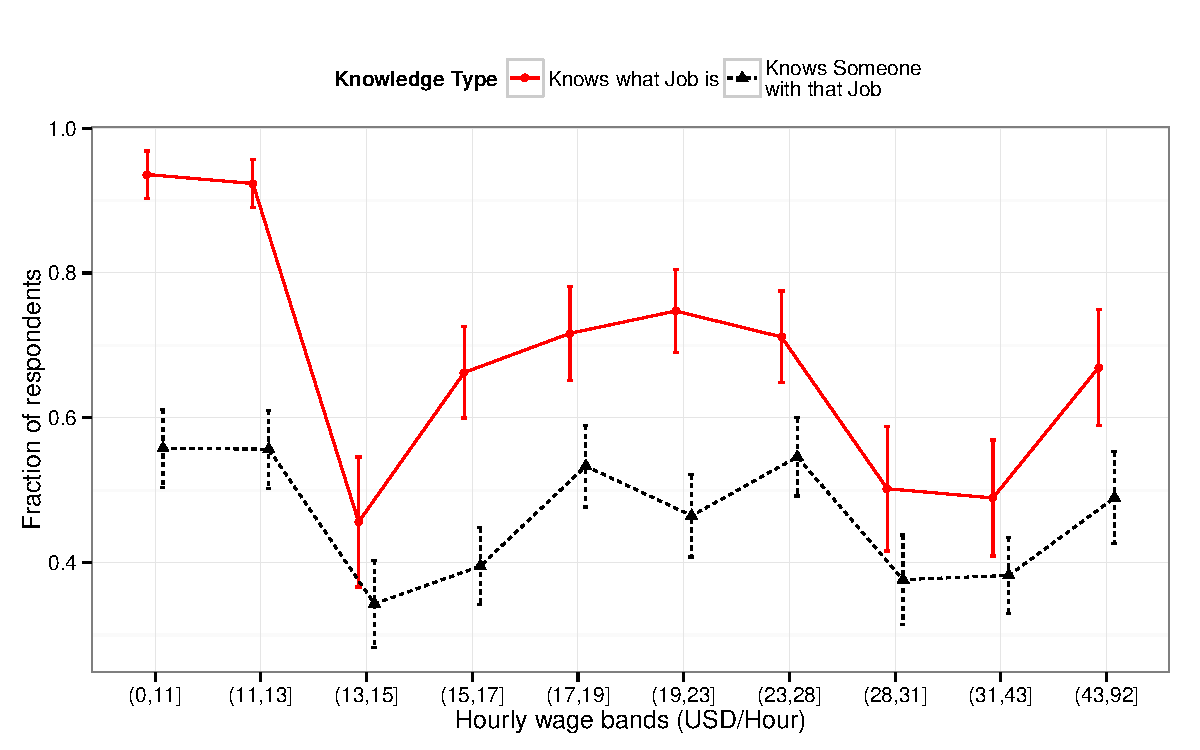
\includegraphics[width = \linewidth]{./plots/knowledge_by_wage.pdf}
% \\
% \emph{Notes:} This figure shows the mean fraction of respondents either knowing someone or knowing what an occupation consists of, by hourly wage bands. 
% \end{minipage}  
% \end{figure} 


% 
% Table created by stargazer v.4.5.3 by Marek Hlavac, Harvard University. E-mail: hlavac at fas.harvard.edu
% Date and time: Sat, Dec 14, 2013 - 07:27:59 AM
\begin{table}[!htbp] \centering 
  \caption{Fixed effects estimation of social knowledge and job knowledge on MSE in log hourly wage predictions} 
  \label{tab:panel_prediction} 
\begin{tabular}{@{\extracolsep{5pt}}lcc} 
\\[-1.8ex]\hline 
\hline \\[-1.8ex] 
 & \multicolumn{2}{c}{\textit{Dependent variable:}} \\ 
\cline{2-3} 
 & MSE of log points & MSE Log wage pct \\ 
\\[-1.8ex] & (1) & (2)\\ 
\hline \\[-1.8ex] 
 Social index & $-$0.039$^{*}$ & $-$0.036$^{*}$ \\ 
  & (0.017) & (0.017) \\ 
  & & \\ 
 Job Knowledge Index & $-$0.022 & $-$0.023 \\ 
  & (0.034) & (0.036) \\ 
  & & \\ 
\hline \\[-1.8ex] 
Observations & 2,951 & 2,951 \\ 
R$^{2}$ & 0.003 & 0.002 \\ 
Adjusted R$^{2}$ & 0.003 & 0.002 \\ 
F Statistic (df = 2; 2850) & 4.014$^{*}$ & 2.958 \\ 
\hline 
\hline \\[-1.8ex] 
\textit{Note:}  & \multicolumn{2}{l}{$^{*}$p$<$0.05; $^{**}$p$<$0.01; $^{***}$p$<$0.001} \\ 
 & \multicolumn{2}{l}{Here are some notes} \\ 
\normalsize 
\end{tabular} 
\end{table} 
  
%\begin{table}[htbp]\centering
\def\sym#1{\ifmmode^{#1}\else\(^{#1}\)\fi}
\caption{Social Knowledge and Labor Market Information Accuracy}
\begin{tabular}{l*{2}{c}}
\hline\hline
            &\multicolumn{1}{c}{(1)}         &\multicolumn{1}{c}{(2)}         \\
            &       error         &       Error         \\
\hline
Social Index&      -0.008         &      -0.047\sym{**} \\
            &     (0.006)         &     (0.017)         \\
Job Knowledge Index&      -0.001         &      -0.025         \\
            &     (0.011)         &     (0.031)         \\
\hline
\(N\)       &        2952         &        2952         \\
\hline\hline
\multicolumn{3}{l}{\footnotesize Standard errors in parentheses}\\
\multicolumn{3}{l}{\footnotesize \sym{*} \(p<0.05\), \sym{**} \(p<0.01\), \sym{***} \(p<0.001\)}\\
\end{tabular}
\end{table}
  



\begin{figure}
\begin{minipage}{0.90 \linewidth}

\includegraphics[width = \linewidth]{./plots/dendrogram.pdf}
\end{minipage}  
\end{figure} 


Social knowledge itself displays an interesting U-shaped pattern: 
workers know people with low wage jobs and high wage jobs, but know far fewer people in middle wage occupations. 
Respondent knowledge is also stratified by occupational income: 
Workers do not know about random subsets of occupations, but instead, knowing more high occupations makes it more likely that the respondent will know some other high wage occupation. 


% TO DO 

% Ask workers for age, gender, income & employment status? 
% Validate against Google consumer surveys 
% Check against variance in that occupation---is greater pct error driven by greater variance? 

%% The sample of workers answering questions on MTurk. 
%% If a pattern or causal effect exists in one population, there is always a question of generalizability. 
%% What if the sample of respondents is just a sample of low-wage workers? 
%% - We can ask workers for their incomes 
%% - We can show in the literature that this is not a particularly biased group 
%% - We can use Google Survey, a nationally representative sample, to adjust 
%% What if high-way jobs are just less common? Controlling for the total employment in that category does not make the effect go away. 
%% What if the hourly/annual salary throws things off? 
%% Do high-way jobs just have more variance? 
%% Was the hourly range top-coded? We started using different binnings that the top, which mechanically reduces predictive accuracy.  
%% Should the panel estimates have clustered standard errors? 
%% Is the BLS 'major' category the right one? The ``Managerial, Other'' type occupations are not really adding much to the analysis. 
%% Turn both knowledge measures into Likert scales 

%% Future work 
%% Wage profile tenure 
%% Link up with representative data 
%% Perhaps one could sample some vacancies as a ``stake in the ground.'' 

%Even when controlling for social knowledge, error percentages increase with the actual wage of the occupation. 
% Preview results 
% Respondent knowledge appears segmented, in that workers 
%% The focus on the analysis was to:
%% -characterize performance and see whether the ``wisdom of crowds'' hypotheses holds regarding occupations 
%% -find poorly labeled occupations in the BLS/OES 
%% -see what occupations are misperceived. 
%% -see how total employment and social knowledge mediate performance in estimating hourly wages 
%% -test whether social knowledge is ``segmented'' by wage  
%% - Idea: break bands, with four drop downs into (0 - 25)(26-50)(51 - 75)(76 - 100)
%% Why are physicains and surgeons ``off'' - is it top-coded? 

% Questions: 
% 1) Are log wages homoscedastic wrt to standard errors? 

%% Granovetter---weak ties. 
%% Some evidence for the Social learning hypotheses.  


% One concern with this study is that results from convenience samples do not necessarily generalize to the larger population. 
% However, convience samples---beyond just being convenient---can given credible results for certain kinds of questions, particularly those trying to detect correlations.
% \footnote{ 
% For example, volunteers for a clinical trial presumably do not have hypertension at the same rate as the population, but if some drug can reduce levels of hypertension in a clinical trial, we suspect that directinal effect would also hold in the population.}


\subsection{Stratification in occupational knowledge by wage} 

A important question is whether workers are stratified in their knowledge about occupational wages. 
If workers only know about wages ``locally'' they might be stuck in a kind of trap, unwilling to make substantial human capital investments without more certainty about the reward.  
We can test partially test this stratification proposition by seeing whether, for each occupation, social knowledge is predicted by the mean wages of the other occupations for which the worker claimed to have social knowledge. 

Consider a worker $i$ evaluating an occupation, $j$. 
This occupation has an actual wage $w_j$. 
Let $S_{ij}$ be an indicator whether $i$ knows someone working in occupation $j$. 
For $S_j$, we compute $\bar{w}^S_{-j}$, which is the mean wage of other occupations for which the worker had social knowledge, knowing someone in that wage.  

In Table~\ref{tab:clustering}, Column~(1), I report an estimate of 
\begin{align} \label{eq:cluster}
\mbox{Pr}\{S_i = 1\} = \alpha + \beta \log w_j + \gamma \log \bar{w}^S_{-j} + \delta \left( \log w_j \times \log \bar{w}^S_{-j} \right) + \epsilon_{ij}. 
\end{align} 

%%%%%%%%%%%%%%%%%%%%%%%%%%%%%%%%%%%%%%%%%%%%%%%%%%%%%%%%%%%%%%%%%%%%%%%%%%%%%%%%%%%%%%%%%%%%%%%%%%%%%%%%%%%%%%%%%%%%%%%%%%%%%%%%%%%%%%%%%%%%%%
%
% Calls:
% (1):  lm(formula = I(social > -2) ~ log(actual.mean.wage) * mean.wage.others.social + log(tot.emp), data = by.worker.df) 
% (2):  lmer(formula = I(social > -2) ~ log(actual.mean.wage) * mean.wage.others.social + log(tot.emp) + (1 | WorkerId), data = by.worker.df) 
% (3):  lmer(formula = I(social > -2) ~ log(actual.mean.wage) * mean.wage.others.social + (1 | WorkerId) + (1 | title), data = by.worker.df) 
%
%%%%%%%%%%%%%%%%%%%%%%%%%%%%%%%%%%%%%%%%%%%%%%%%%%%%%%%%%%%%%%%%%%%%%%%%%%%%%%%%%%%%%%%%%%%%%%%%%%%%%%%%%%%%%%%%%%%%%%%%%%%%%%%%%%%%%%%%%%%%%%
\begin{tabular}{lcD{.}{.}{7}cD{.}{.}{7}cD{.}{.}{7}}
\toprule
&&\multicolumn{1}{c}{(1)} && \multicolumn{1}{c}{(2)} && \multicolumn{1}{c}{(3)}\\
\midrule
(Intercept)                                             &  &  3.574^{***} &&  2.699^{**}  &&  4.880^{***}\\
                                                        &  &  (1.015)     &&  (0.977)     &&  (0.929)    \\
log(actual.mean.wage)                                   &  & -1.510^{***} && -1.244^{***} && -1.390^{***}\\
                                                        &  &  (0.327)     &&  (0.306)     &&  (0.296)    \\
mean.wage.others.social                                 &  & -1.626^{***} && -1.318^{***} && -1.406^{***}\\
                                                        &  &  (0.332)     &&  (0.320)     &&  (0.307)    \\
log(tot.emp)                                            &  &  0.131^{***} &&  0.131^{***} &&             \\
                                                        &  &  (0.015)     &&  (0.014)     &&             \\
log(actual.mean.wage) $\times$ mean.wage.others.social &  &  0.504^{***} &&  0.415^{***} &&  0.447^{***}\\
                                                        &  &  (0.109)     &&  (0.102)     &&  (0.098)    \\
Var((Intercept)|WorkerId)                               &  &              &&   0.045      &&   0.040     \\
                                                        &  &              &&              &&             \\
Var(|Residual)                                          &  &              &&   0.198      &&   0.179     \\
                                                        &  &              &&              &&             \\
Var((Intercept)|title)                                  &  &              &&              &&   0.027     \\
                                                        &  &              &&              &&             \\
\midrule
R-squared                                               &  &      0.040   &&              &&             \\
adj. R-squared                                          &  &      0.039   &&              &&             \\
sigma                                                   &  &      0.489   &&              &&             \\
F                                                       &  &     26.252   &&              &&             \\
p                                                       &  &      0.000   &&              &&             \\
Log-likelihood                                          &  &  -1754.623   &&  -1609.371   &&  -1555.602  \\
Deviance                                                &  &    596.067   &&   3218.743   &&   3111.204  \\
AIC                                                     &  &   3521.245   &&   3232.743   &&   3125.204  \\
BIC                                                     &  &   3556.182   &&   3273.503   &&   3165.964  \\
N                                                       &  &   2497       &&   2497       &&   2497      \\
\bottomrule
\end{tabular}
 

As we saw earlier, knowledge is decreasing in the wage of the occupation, in that $\hat{\beta}$ is negative. 
Consistent with the stratification hypotheses, the coefficient on the acutal wage and the social knowedge wage is positive, or $\hat{\delta} > 0$. 
Respondents that reported knowing people in higher-wage occupation where more likely to know someone in the $i$th occupation if the $i$th occupation was itself higher-wage. 
In Column~(2), as a falsification test I report the same regression as in Equation~\ref{eq:cluster}, but within each worker, shuffling their social index at random. 
Reassuringly, none of the coefficients are conventionally significant. 
